
\documentclass[11pt,fleqn]{article} 
\usepackage[margin=0.8in, head=0.8in]{geometry} 
\usepackage{amsmath, amssymb, amsthm}
\usepackage{fancyhdr} 
\usepackage{palatino, url, multicol}
\usepackage{graphicx, pgfplots} 
\usepackage[all]{xy}
\usepackage{polynom} 
%\usepackage{pdfsync} %% I don't know why this messes up tabular column widths
\usepackage{enumerate}
\usepackage{framed}
\usepackage{setspace}
\usepackage{array,tikz}

\pgfplotsset{compat=1.6}

\pgfplotsset{soldot/.style={color=black,only marks,mark=*}} \pgfplotsset{holdot/.style={color=black,fill=white,only marks,mark=*}}


\pagestyle{fancy} 
\lfoot{Uses a calculator}
\rfoot{2-2 The Limit of a Function}

\begin{document}
\renewcommand{\headrulewidth}{0pt}
\newcommand{\blank}[1]{\rule{#1}{0.75pt}}
\newcommand{\bc}{\begin{center}}
\newcommand{\ec}{\end{center}}
\renewcommand{\d}{\displaystyle}

\vspace*{-0.7in}

%%%%%%%%%intro page
\begin{center}
  \LARGE
  \sc{Section 2-2: The Limit of a Function}\\
\end{center}
Read Section 2.2. Work the embedded problems. \\
\hrulefill

\begin{enumerate}

\item \fbox{{\sc{example 1:}}} What does the function $f(x) = \frac{x-2}{x^2-x-2}$ look like around $x=2$?

\vfill

\item \fbox{{\sc{example 2:}}} What does the function $f(x) = \frac{2|x-5|}{(x-5)}$ look like around $x=5$?
\vfill
\newpage
\item \fbox{{\sc{definition:}}} two-sided limit

Say: ``the limit of $f(x)$, as $x$ approaches $a$ is $L$"\\

Write: \\

It means: \\
\vspace{0.5in}

\item \fbox{{\sc{definition:}}} one-sided limits
	\begin{itemize}

	\item Say: ``the limit of $f(x)$, as $x$ approaches $a$ \emph{on the left} is $L$ "\\

Write: \\

It means: \\
\vspace{0.5in}

	\item Say: ``the limit of $f(x)$, as $x$ approaches $a$ \emph{on the right} is $L$ "\\

Write: \\

It means: \\
\vspace{0.5in}
	\end{itemize}
	
\item \fbox{{\sc{example 3:}}} What does the function $f(x) = \frac{8-x}{(x-2)^2}$ look like around $x=2$?
\vfill

\item \fbox{{\sc{definition:}}} infinite limits\\

\vspace{.3in}
\newpage

%%%COMMENT OUT TO STUDENTS
%\begin{tabular}{|c|c|c|c|c|c|c|c|c|c|c|c|}
%$x$&1&1.5&1.9&1.99&1.999&2&2.001&2.01&2.1&2.5&3\\
%\hline
%$f(x)$&0.5&0.4&0.34483&0.33445&0.33344&DNE&0.33322&0.33223&0.32258&0.28571&0.25\\
%\end{tabular}
%\vfill
%What does the table above tell you about the \emph{graph} of $y= \frac{x-2}{x^2-x-2}$?
%\vfill
%
%\newpage
%
%%%BASIC CALCULATION DEMONSTRATION
%
%\fbox{{\sc{example 2:}}} [Why do all the calculation? Just pick a number really close to ``a,''  right???!!] \\
%
%\vspace{0.2in}
%
%\bc Use calculation to guess $\d{\lim_{t \to 0} \frac{\sqrt{t^2+9}-3}{t^2}}.$ \ec
%
%\vspace{0.2in}
%
% Let's just pick numbers super-close to $a=0$, say $\pm 0.000001:$ 
%\begin{tabular}{|c|c|c|c|}
%$t$&-0.000001&0&0.000001\\
%\hline
%$f(t)$&&DNE&\\
%\end{tabular}
%
%\vspace{0.2in}
%
%Hint: Always be skeptical! Why can't this be right and what went wrong?
%\vfill
%
%\fbox{{\sc{example 3:}}} [Sample points may not illustrate the big picture. Theory will be useful.]\\
%
%\bc Use calculation to guess $\d{\lim_{\theta \to 0} \sin \left(\frac{\pi}{\theta}\right)}.$ \ec
%
%\begin{tabular}{|c|c|c|c|c|c|c|c|}
%$x$&-0.1&-0.001&-0.0001&0&0.0001&0.001&0.01\\
%\hline
%$f(x)$&&&&&&&\\
%\end{tabular}
%\quad \quad Do you believe your answer?
%\vfill
%\newpage
%
%%%STARTER PRACTICE
%
%\begin{center} Practice Problems \end{center}
%\begin{enumerate}
%\item For each problem below, fill out the chart of values, then use the values to \emph{guess} the value of the limit. Finally rate your confidence level on a 0 to 3 scale where ( 0 = I'm sure this is wrong ) and (3 = I'm  sure this is right.)
%\begin{enumerate}
%%Example from book
%\item $\displaystyle{\lim_{\theta \to 0}} \frac{\sin \theta}{\theta}= \framebox(20,20){}$ \hfill confidence? \underline{\hspace{.5in}}\\
%\begin{tabular}{|c| m{0.6cm} | m{0.6cm} | m{0.6cm} | m{0.6cm} | m{0.6cm} | c | m{0.6cm} | m{0.6cm} |m{0.6cm} |m{0.6cm} | m{0.6cm} |}
%\hline
%$x$&&&&&&0&&&&&\\
%\hline
%&&&&&&&&&&&\\
%$f(x)$&&&&&&&&&&&\\
%&&&&&&&&&&&\\
%\hline
%\end{tabular}
%\vfill
%%piecewise
%\item $\displaystyle{\lim_{x \to 2}} f(x) = \framebox(20,20){}$ where
%$\begin{cases} |x-1| & x \leq 2  \\ x+1 & x > 2 \end{cases}$ \hfill confidence? \underline{\hspace{.5in}}\\
%\begin{tabular}{|c| m{0.6cm} | m{0.6cm} | m{0.6cm} | m{0.6cm} | m{0.6cm} | c | m{0.6cm} | m{0.6cm} |m{0.6cm} |m{0.6cm} | m{0.6cm} |}
%\hline
%$x$&&&&&&2&&&&&\\
%\hline
%&&&&&&&&&&&\\
%$f(x)$&&&&&&&&&&&\\
%&&&&&&&&&&&\\
%\hline
%\end{tabular}
%\vfill
%%\item $\displaystyle{\lim_{x \to}}=$ \hfill confidence? \underline{\hspace{.5in}}\\
%%\begin{tabular}{|c|c|c|c|c|c|c|c|c|c|c|c|}
%%\hline
%%$x$&&&&&&&&&&&\\
%%\hline
%%&&&&&&&&&&&\\
%%$f(x)$&&&&&&&&&&&\\
%%&&&&&&&&&&&\\
%%\hline
%%\end{tabular}
%%infinite limit
%\item $\displaystyle{\lim_{x \to 0} \frac{e^{2x}-1}{x}}= \framebox(20,20){}$ \hfill confidence? \underline{\hspace{.5in}}\\
%\begin{tabular}{|c|c|c|c|c|c|c|c|c|c|c|c|}
%\hline
%$x$& \quad -0.5 \quad & \quad -0.1 \quad &-0.01&-0.001&-0.0001&0&0.0001&0.001&0.01& \quad 0.1 \quad & \quad 0.5 \quad \\
%\hline
%&&&&&&&&&&&\\
%$f(x)$&&&&&&&&&&&\\
%&&&&&&&&&&&\\
%\hline
%\end{tabular}
%\vfill
%\end{enumerate}
%\newpage
%
%%%INTRO TO ONE_SIDED LIMITS
%\fbox{\sc{Definitions:}} 
%
%Say: ``the limit as $x$ approaches $a$ \emph{on the left} is $L$"; \hfill Write: \framebox(120,30){}\\
%
%It means \\
%
%\vspace{.5in}
%
%Say: ``the limit as $x$ approaches $a$ \emph{on the right} is $L$"; \hfill Write: \framebox(120,30){}\\
%
%It means \\
%
%\vspace{.5in}

\item The function $g(x)$ is graphed below. Use the graph to fill in the blanks.

\begin{tabular}{m{9cm}  c m{5cm}}
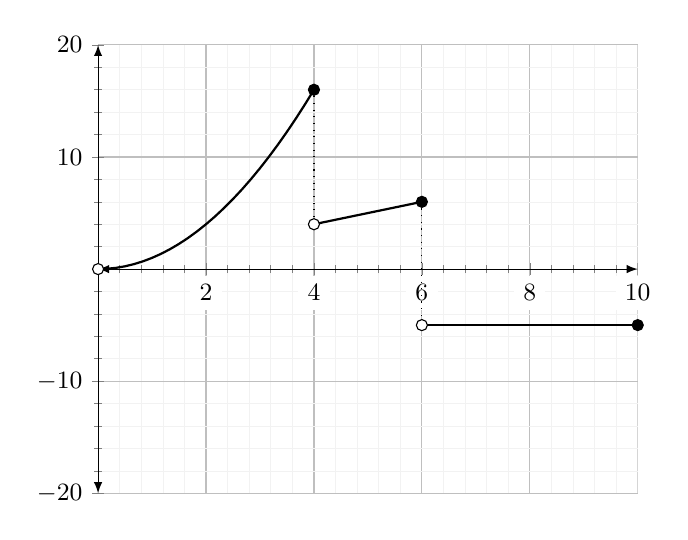
\begin{tikzpicture}[scale=1]
\begin{axis}[grid style={line width=.2pt, draw=gray!10},grid=both,major grid style={line width=.4pt,draw=gray!50},
    xmin=0,xmax=10,
    ymin=-20,ymax=20,
    xtick={},ytick={},
    minor tick num=4,
    enlargelimits={abs=0},
    ticklabel style={font=\small,fill=white},
    axis lines=middle,
    axis line style={latex-latex},
    xlabel style={at={(ticklabel* cs:1)},anchor=north west},
    ylabel style={at={(ticklabel* cs:1)},anchor=south west}
]
\addplot[domain=0:4,black, thick] {x*x};
\addplot[domain=4:6,black, thick] {x};
\addplot[domain=6:10,black, thick] {-5};
\draw[dotted] (axis cs:4,16) -- (axis cs:4,4);
\draw[dotted] (axis cs:6,6) -- (axis cs:6,-5);
\addplot[holdot] coordinates{(0,0)(4,4)(6,-5)};
\addplot[soldot] coordinates{(4,16)(6,6)(10,-5)};
\end{axis}
\end{tikzpicture}
& \quad &
\begin{enumerate}
\item$\d{\lim_{x \to 4^-} f(x) = \underline{\hspace{2cm}} }$
\item$\d{\lim_{x \to 4^+} f(x) = \underline{\hspace{2cm}} }$
\item$\d{\lim_{x \to 4} f(x) = \underline{\hspace{2cm}} }$
\item $f(4)= \underline{\hspace{2cm}}$
\item $\d{\lim_{x \to 8} f(x) = \underline{\hspace{2cm}} }$
\item $f(8)= \underline{\hspace{2cm}}$
\end{enumerate}
\end{tabular}

\item The function $g(x)$ is graphed below. Use the graph to fill in the blanks.

\begin{tabular}{m{9cm}  c m{5cm}}
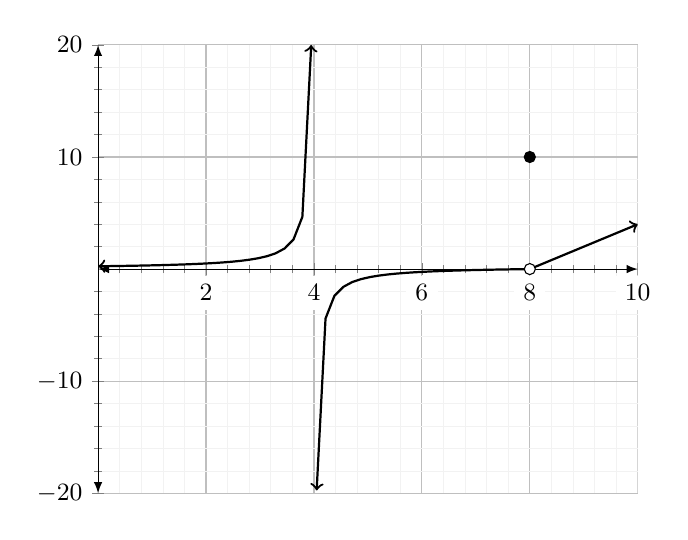
\begin{tikzpicture}[scale=1]
\begin{axis}[grid style={line width=.2pt, draw=gray!10},grid=both,major grid style={line width=.4pt,draw=gray!50},
    xmin=0,xmax=10,
    ymin=-20,ymax=20,
    xtick={},ytick={},
    minor tick num=4,
    enlargelimits={abs=0},
    ticklabel style={font=\small,fill=white},
    axis lines=middle,
    axis line style={latex-latex},
    xlabel style={at={(ticklabel* cs:1)},anchor=north west},
    ylabel style={at={(ticklabel* cs:1)},anchor=south west}
]

\addplot[<->,domain=0:3.95,black, thick] {(4-x)^(-1)};
\addplot[<-,domain=4.05:8,black, thick] {(4-x)^(-1)+0.25};
\addplot[->,domain=8:10,black, thick] {2*x-16};
%\draw[dotted] (axis cs:4,16) -- (axis cs:4,4);
%\draw[dotted] (axis cs:6,6) -- (axis cs:6,-5);
\addplot[soldot] coordinates{(8,10)};
\addplot[holdot] coordinates{(8,0)};
\end{axis}
\end{tikzpicture}
& \quad &
\begin{enumerate}
\item$\d{\lim_{x \to 4^-} f(x) = \underline{\hspace{2cm}} }$
\item$\d{\lim_{x \to 4^+} f(x) = \underline{\hspace{2cm}} }$
\item$\d{\lim_{x \to 4} f(x) = \underline{\hspace{2cm}} }$
\item $f(4)= \underline{\hspace{2cm}}$
\item $\d{\lim_{x \to 8} f(x) = \underline{\hspace{2cm}} }$
\item $f(8)= \underline{\hspace{2cm}}$
\end{enumerate}
\end{tabular}

Write the equation of any vertical asymptote:

\item What is the relationship between limits and vertical asymptoes?
\vspace{1in}
\newpage
\item Sketch the graph of an function that satisfies \emph{all} of the given conditions. \\
\begin{tabular}{lll}
&&\\
$\displaystyle{\lim_{x \to 0^-} f(x)=1}$& $\displaystyle{\lim_{x \to 0^+ }f(x)=-2}$ &$\displaystyle{\lim_{x \to 4^-}f(x)=3}$\\ 
&&\\
$\displaystyle{\lim_{x \to 4^+ }f(x)=0}$& $f(0)=-2$ &$f(4)=1$\\
\end{tabular}
\vspace{2in}

\item Some General Principles
	\begin{multicols}{3}
	\begin{enumerate}
	\item $\displaystyle{\lim_{x \to 0^-} \frac{1}{x} =}$
	\item $\displaystyle{\lim_{x \to 0^+} \frac{1}{x} =}$
	\item $\displaystyle{\lim_{x \to 0} \frac{1}{x} =}$
	\item $\displaystyle{\lim_{x \to 0^-} \frac{1}{x^2} =}$
	\item $\displaystyle{\lim_{x \to 0^+} \frac{1}{x^2} =}$
	\item $\displaystyle{\lim_{x \to 0} \frac{1}{x^2} =}$
	\item $\displaystyle{\lim_{x \to a^-} \frac{1}{x-a} =}$
	\item $\displaystyle{\lim_{x \to a^+} \frac{1}{x-a} =}$
	\item $\displaystyle{\lim_{x \to a} \frac{1}{x-a} =}$
	\end{enumerate}
	\end{multicols}
\end{enumerate}
\end{document}

\item Sketch the graph of an function that satisfies \emph{all} of the given conditions. Compare your answer with that of your neighbor.\\
\begin{tabular}{lll}
&&\\
$\displaystyle{\lim_{x \to 0^-} f(x)=1}$& $\displaystyle{\lim_{x \to 0^+ }f(x)=-2}$ &$\displaystyle{\lim_{x \to 4^-}f(x)=3}$\\ 
&&\\
$\displaystyle{\lim_{x \to 4^+ }f(x)=0}$& $f(0)=-2$ &$f(4)=1$\\
\end{tabular}
\vspace{2in}
\item Determine the limit. Explain your answer.
\begin{enumerate}
\item $\displaystyle{\lim_{x \to 5^+}\frac{2+x}{x-5}}$\\
\vfill
\item $\displaystyle{\lim_{x \to 5^+}\frac{2+x}{5-x}}$\\
\vfill
\item $\displaystyle{\lim_{x \to (\pi/2)^+} \frac{\sec x}{x}}$\\
\vfill
\end{enumerate}
\end{enumerate}
\end{document}

